% ******************************* Thesis Appendix C ********************************

\chapter{Register Transfer Level Design View}
\label{appendix:3}
\section{Design of the First Version}
\label{appendix:3:section:1}
\begin{figure}[]
\centering
%\hspace{3.0cm}
%\vspace{-5cm}
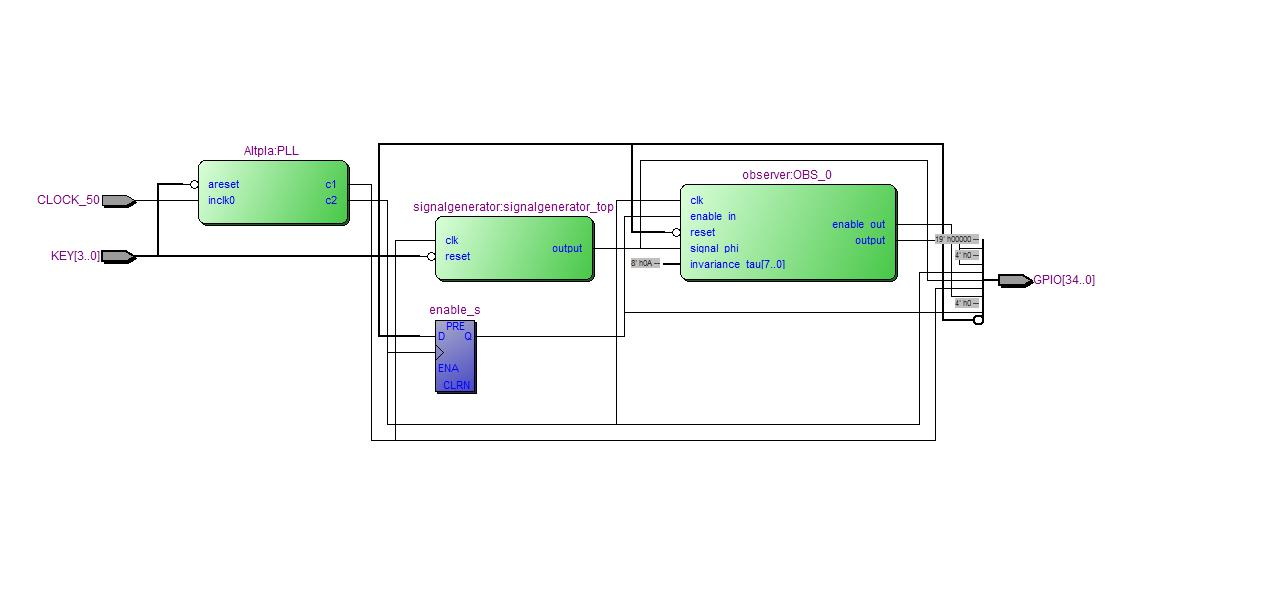
\includegraphics[width=650px,height=300px,angle=-90]{../../pictures/20.02.2014/TOP.jpg}
%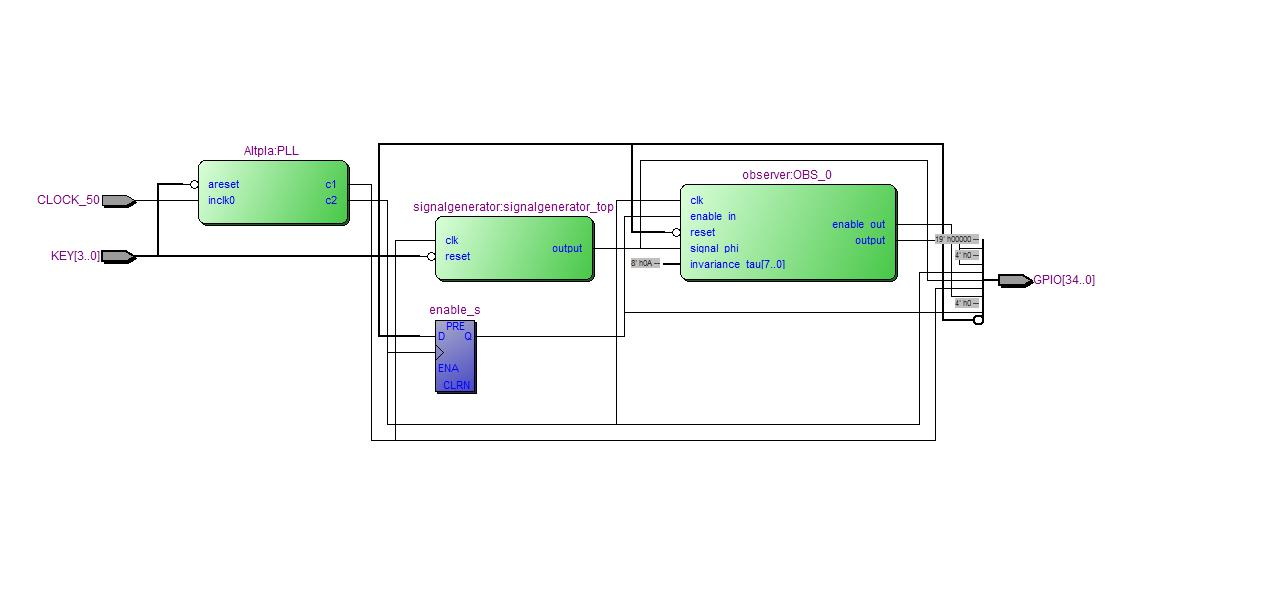
\includegraphics[height]{../../pictures/20.02.2014/TOP.jpg}
\caption[TOP Design of the First Version]{Illustration of the TOP Design of the first correct version,but without improvements}
\label{fig:version:one:top}
\end{figure}

\begin{figure}[]
\centering
%\hspace{3.0cm}
%\vspace{-5cm}
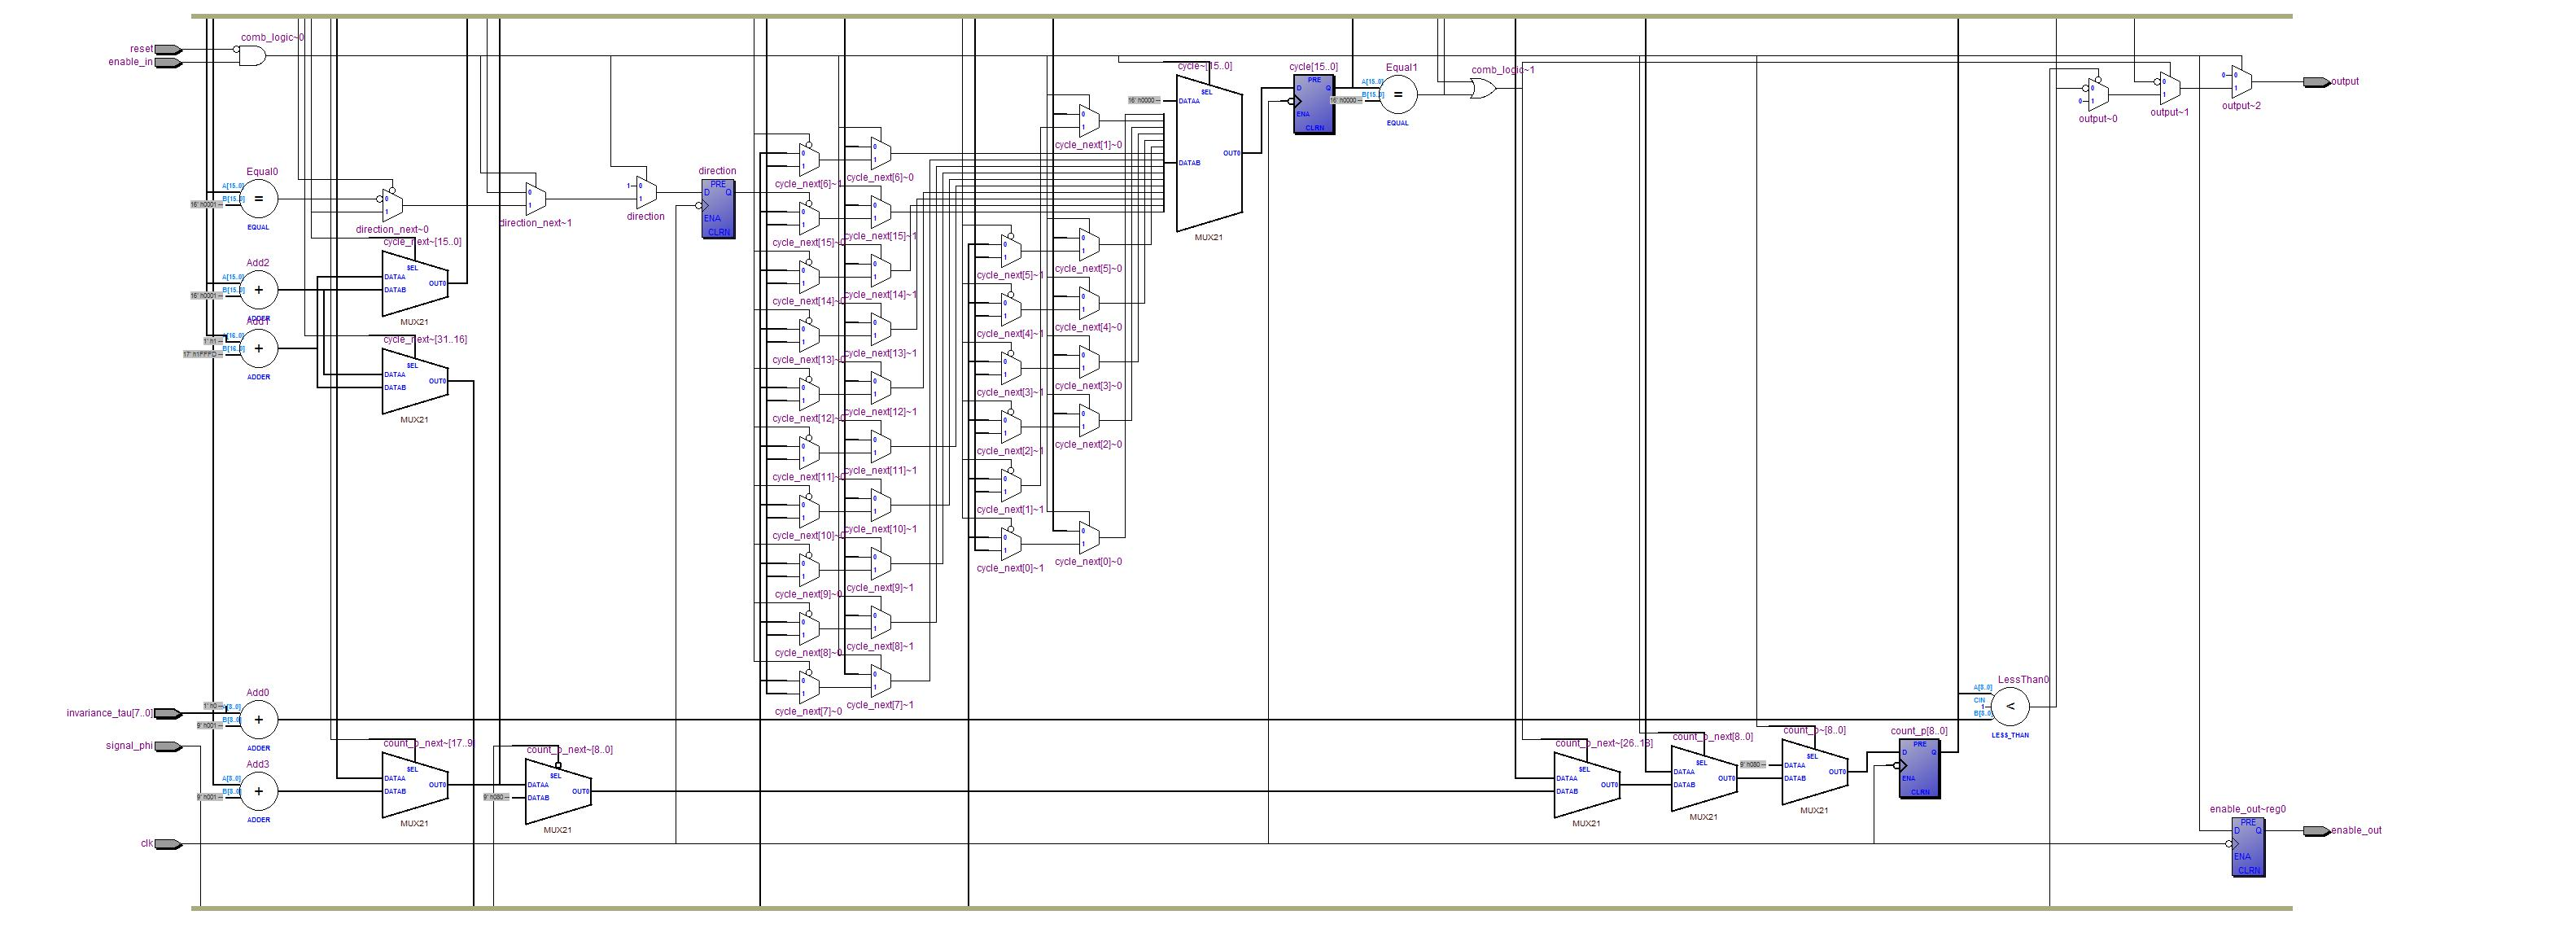
\includegraphics[width=650px,height=300px,angle=-90]{../../pictures/20.02.2014/observer_OBS_0.jpg}
%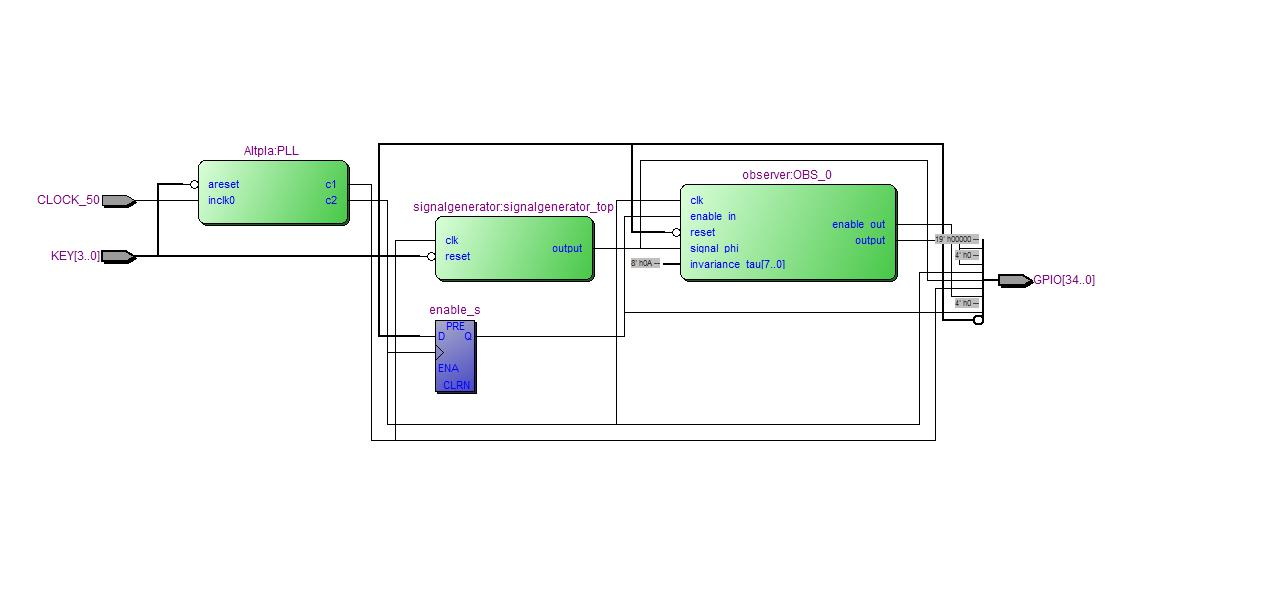
\includegraphics[height]{../../pictures/20.02.2014/TOP.jpg}
\caption[Observer Design of the First Version]{Illustration of the Observer Design of the first correct version,but without improvements}
\label{fig:version:one:obs}
\end{figure}

\begin{figure}[]
\centering
%\hspace{3.0cm}
%\vspace{-5cm}
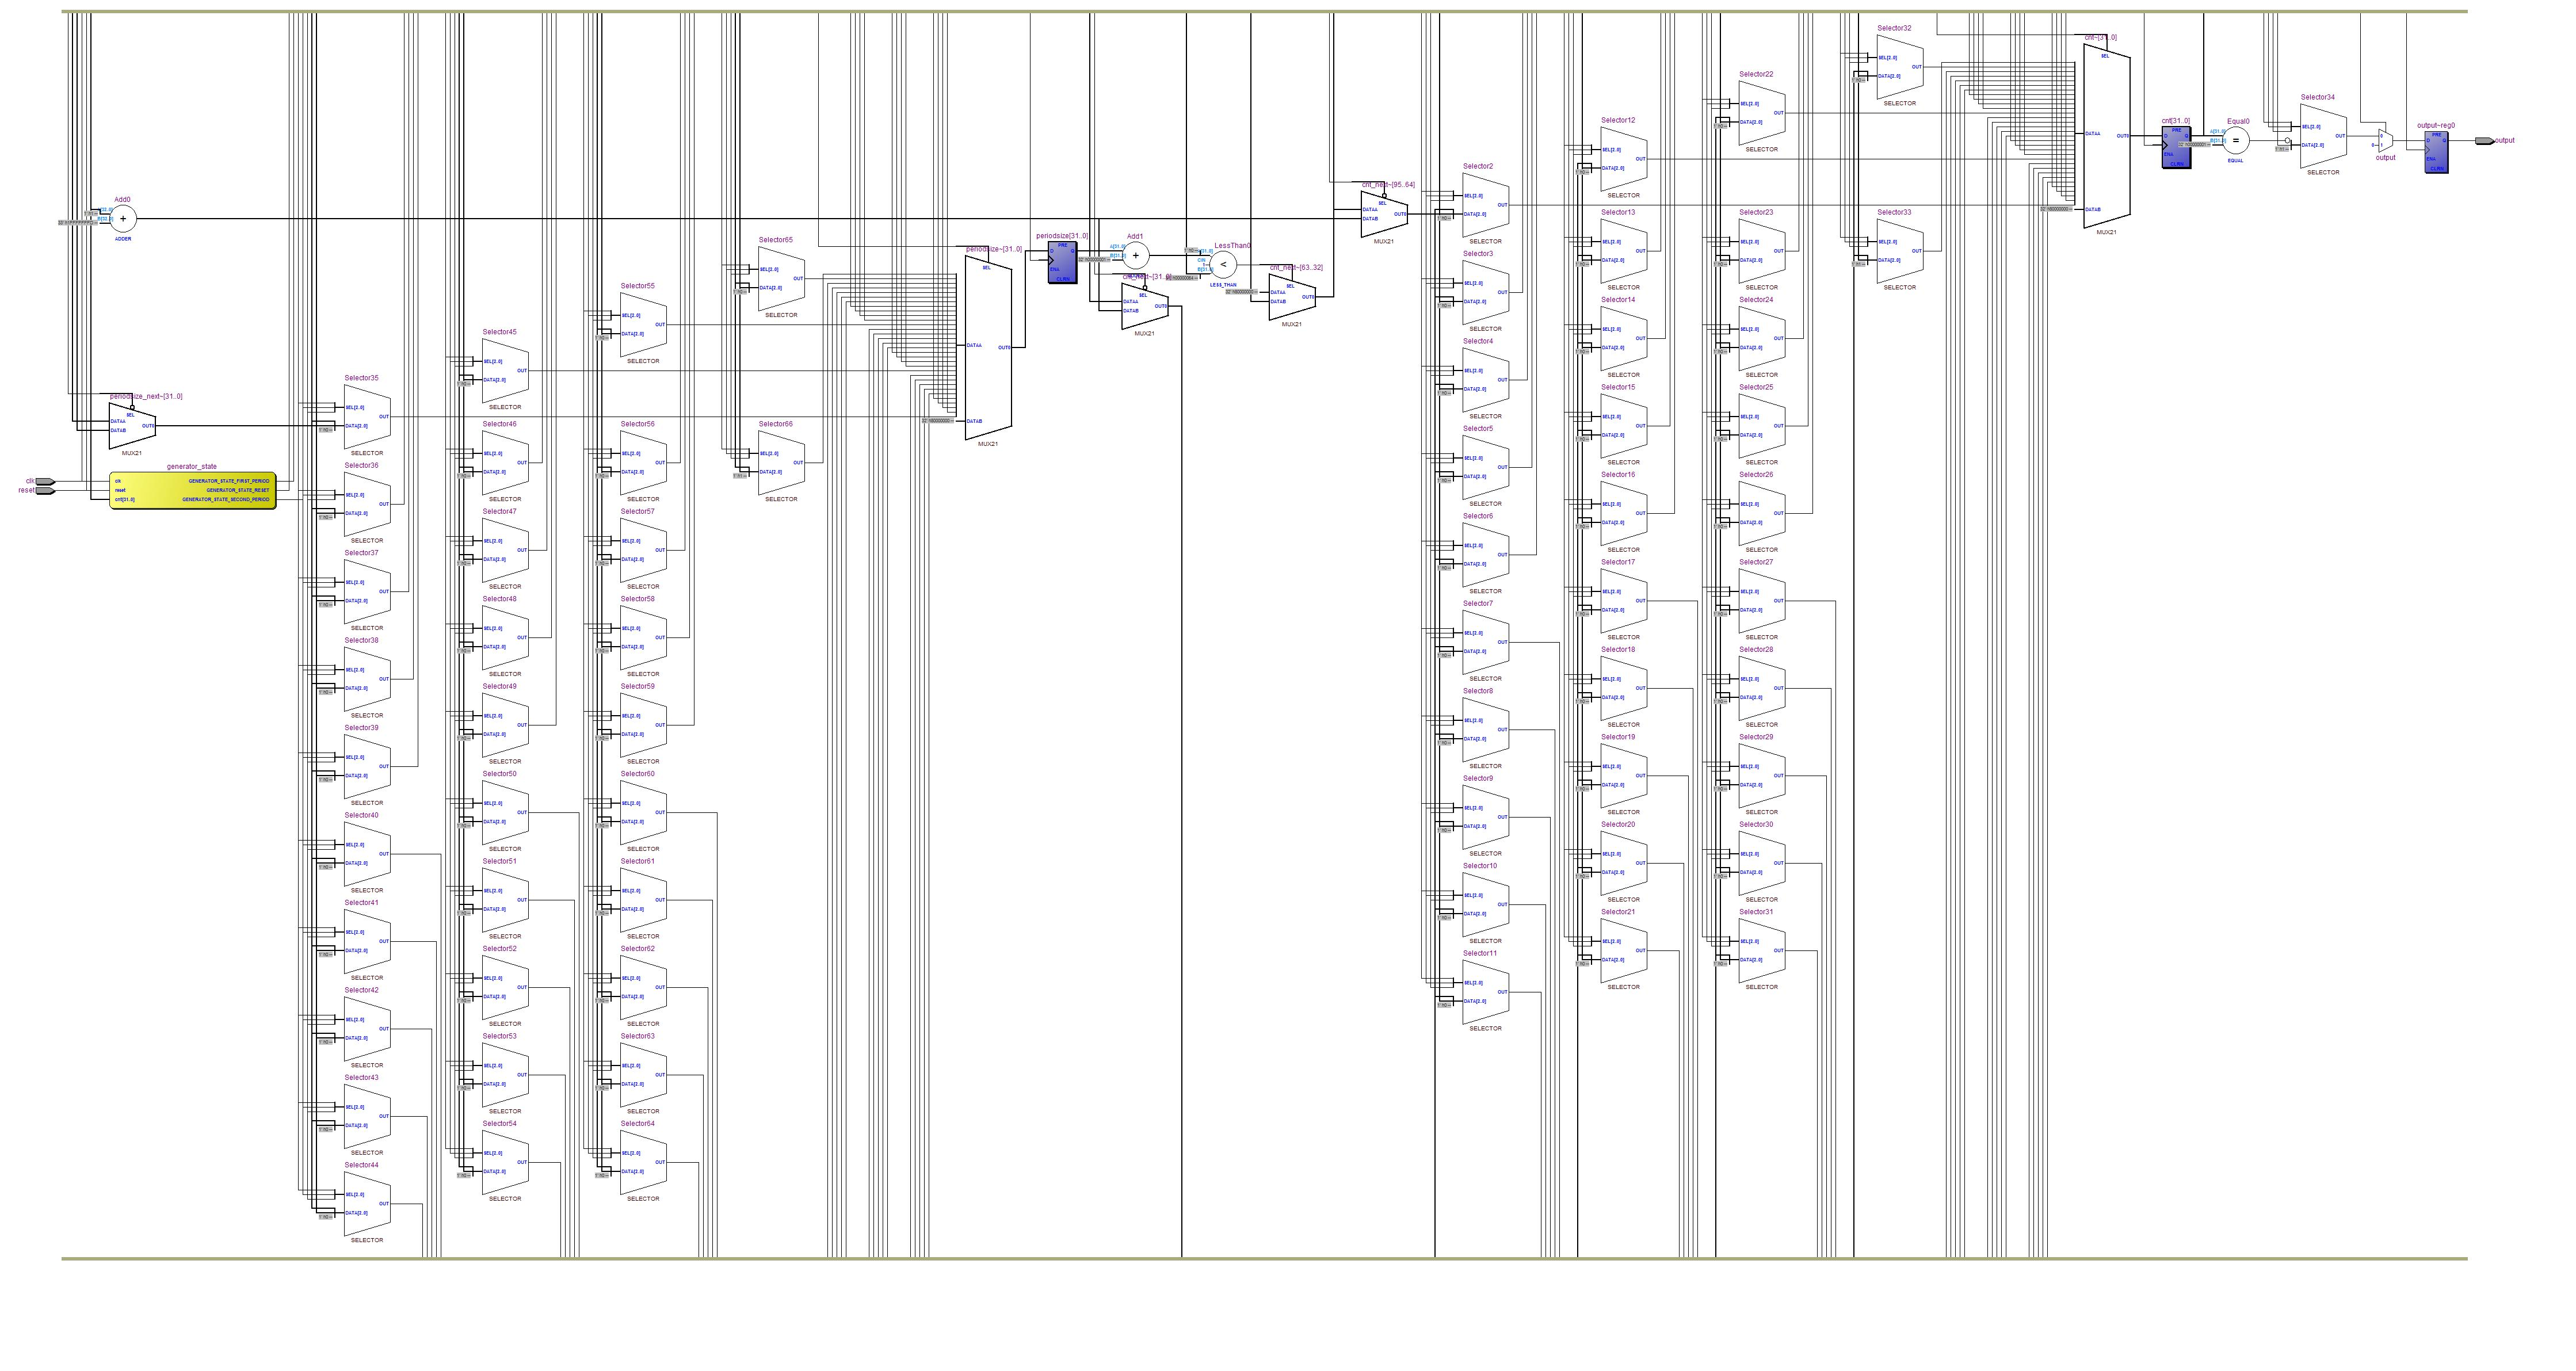
\includegraphics[width=650px,height=300px,angle=-90]{../../pictures/20.02.2014/signalgenerator_signalgenerator_top.jpg}
%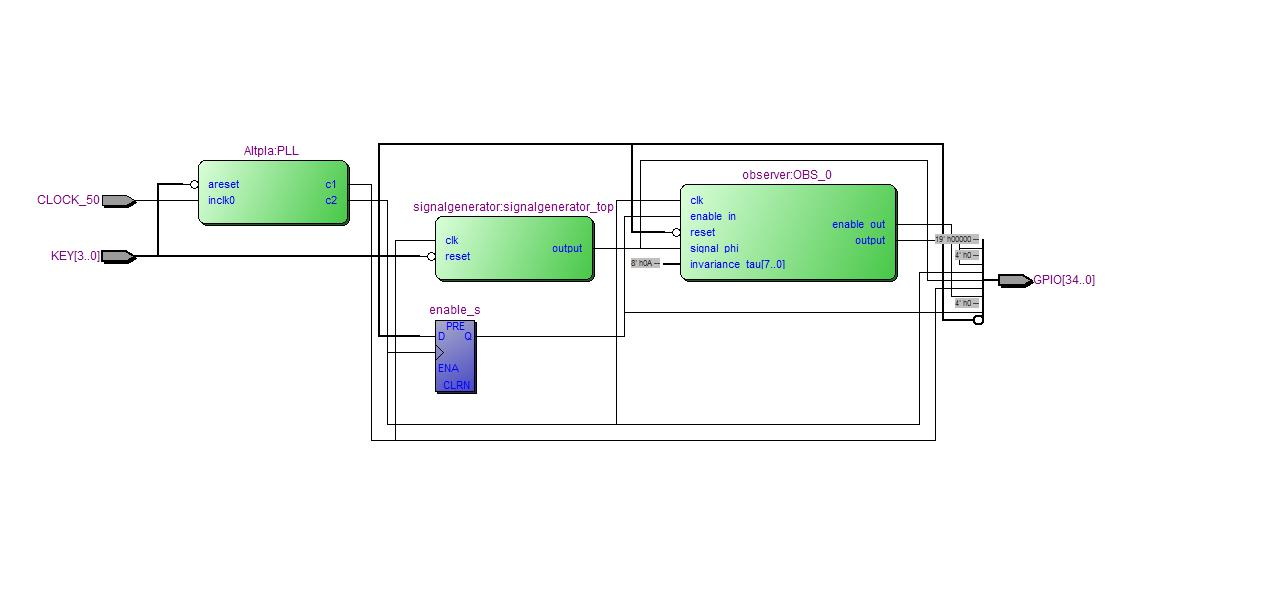
\includegraphics[height]{../../pictures/20.02.2014/TOP.jpg}
\caption[Signalgenerator of the First Version]{Illustration of the Signalgenerator of the first correct version,but without improvements}
\label{fig:version:one:sig}
\end{figure}

\clearpage
\section{Design of the most performant Version}
\label{appendix:3:section:2}


\begin{figure}[]
\centering
%\hspace{3.0cm}
%\vspace{-5cm}
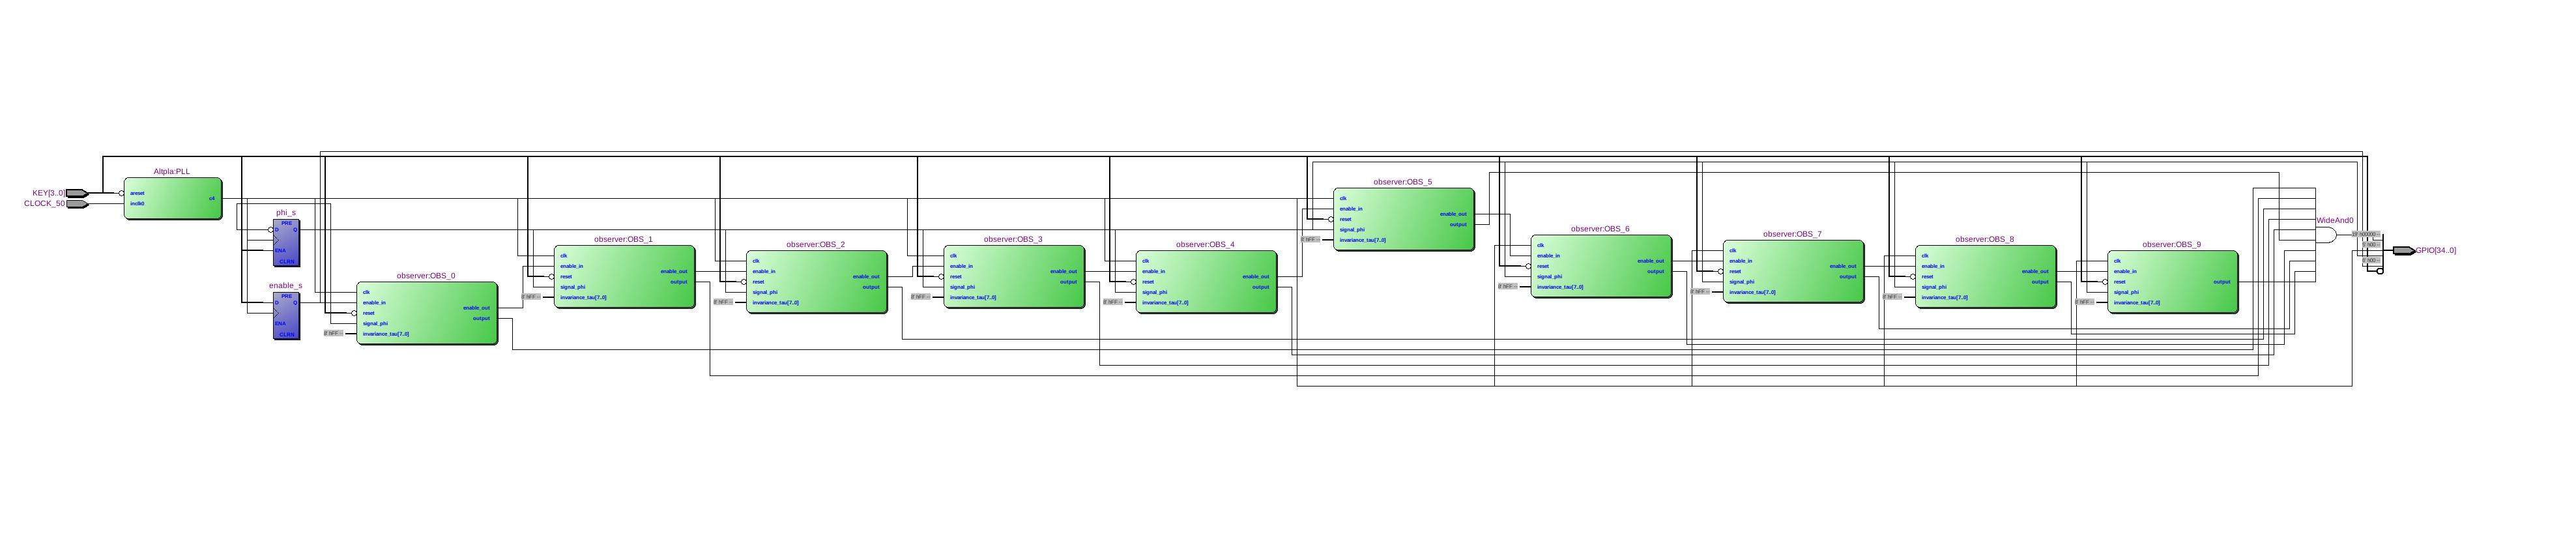
\includegraphics[width=650px,height=300px,angle=-90]{../../pictures/13.06.2014/plain_generator/200Mhz/10OBS/TOP_only_10Observer.jpg}
%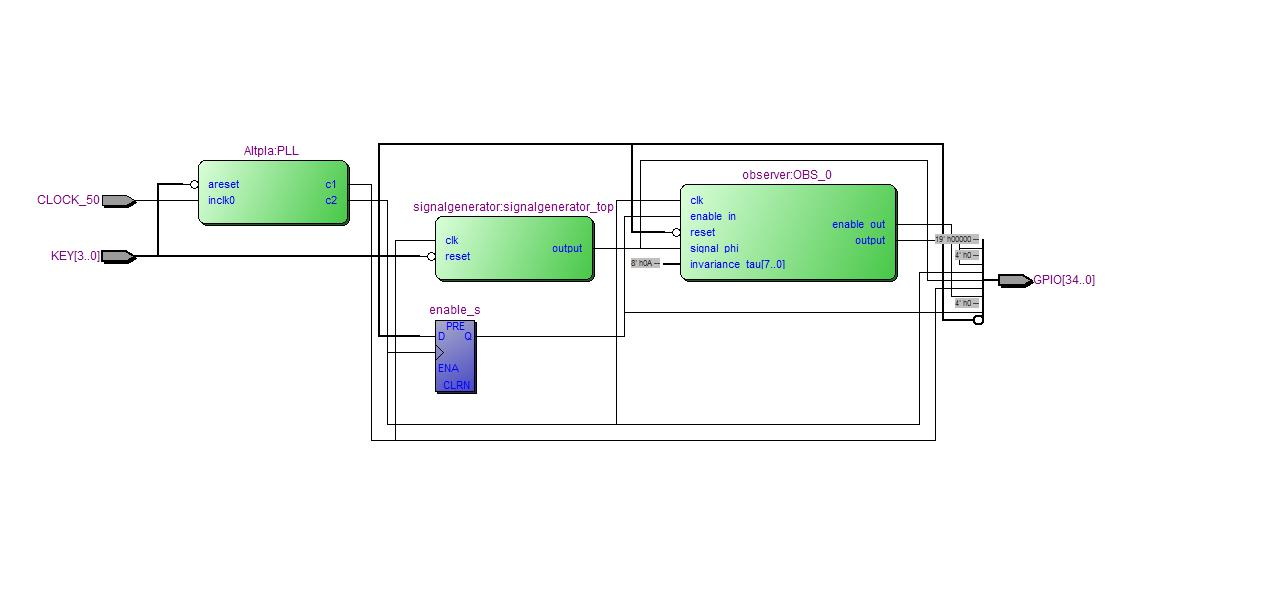
\includegraphics[height]{../../pictures/20.02.2014/TOP.jpg}
\caption[TOP Design of the Final Version]{Illustration of the TOP Design with the the best performance}
\label{fig:version:final:top}
\end{figure}

\begin{figure}[]
\centering
%\hspace{3.0cm}
%\vspace{-5cm}
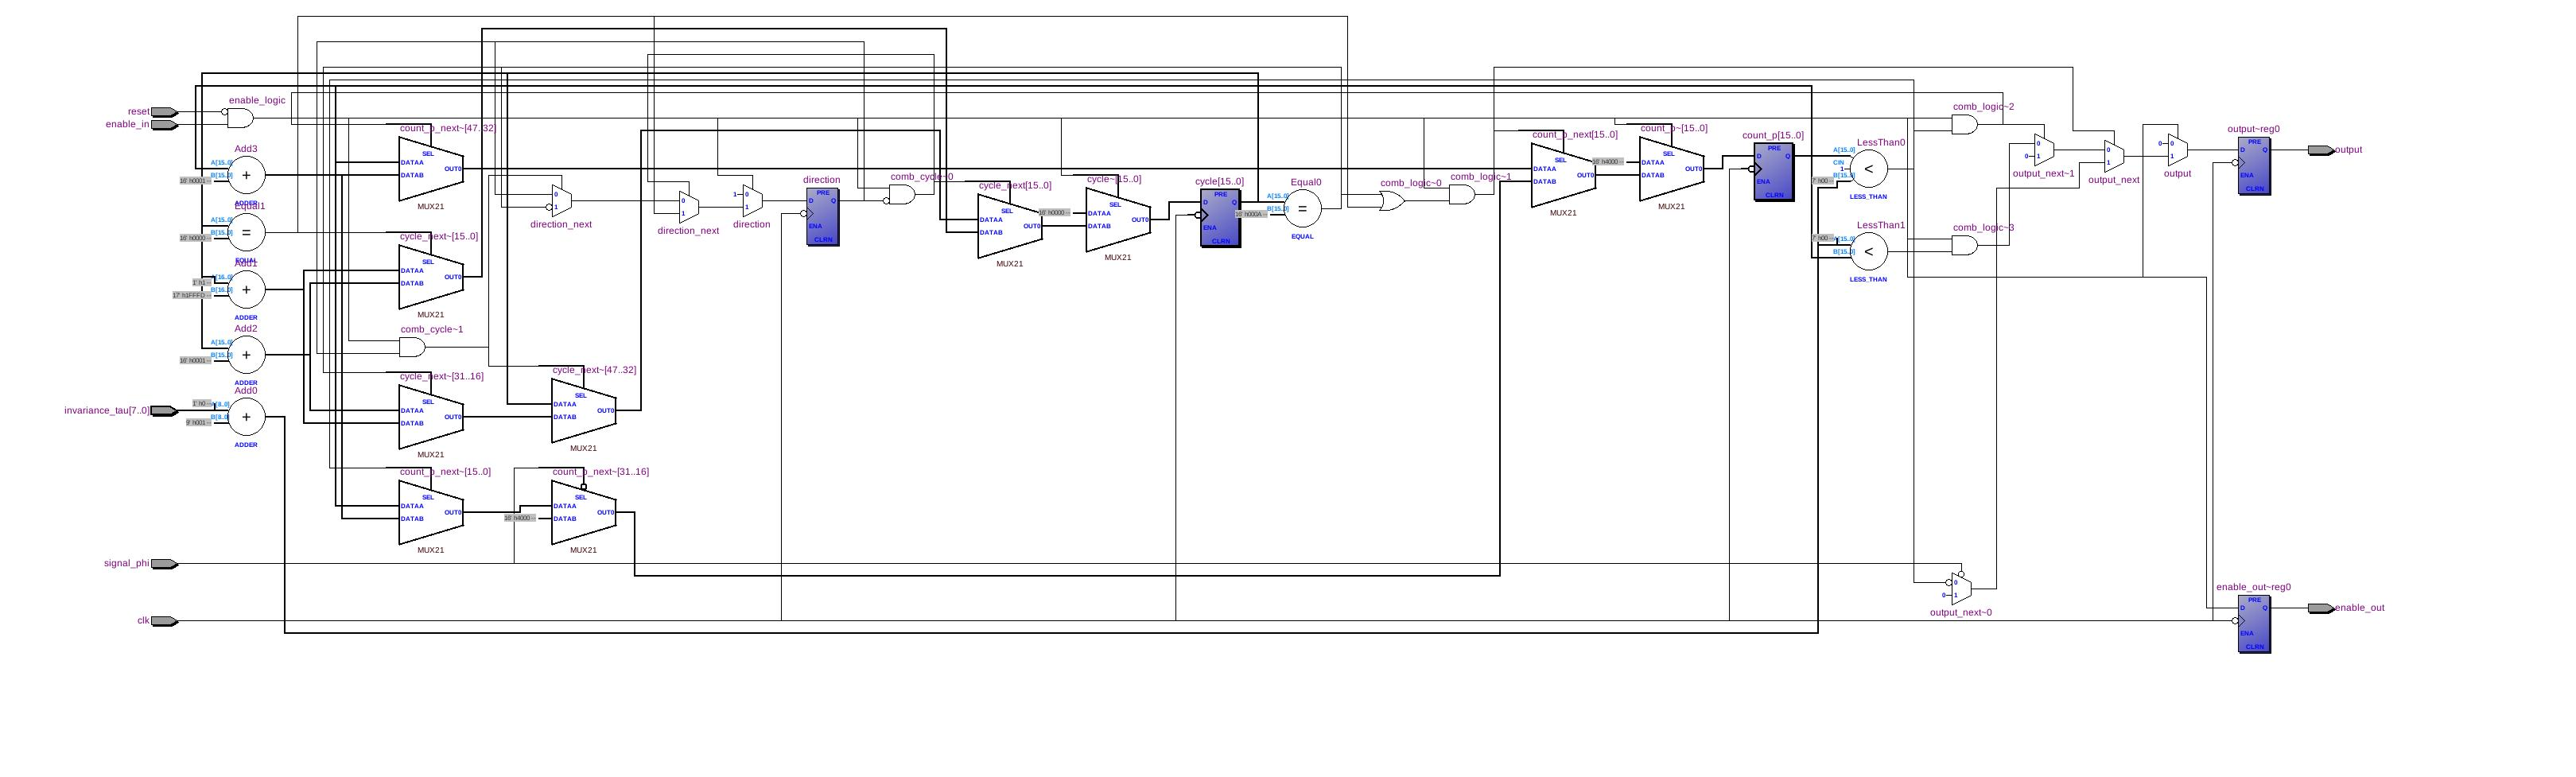
\includegraphics[width=650px,height=300px,angle=-90]{../../pictures/13.06.2014/plain_generator/200Mhz/10OBS/observer_OBS_0.jpg}
%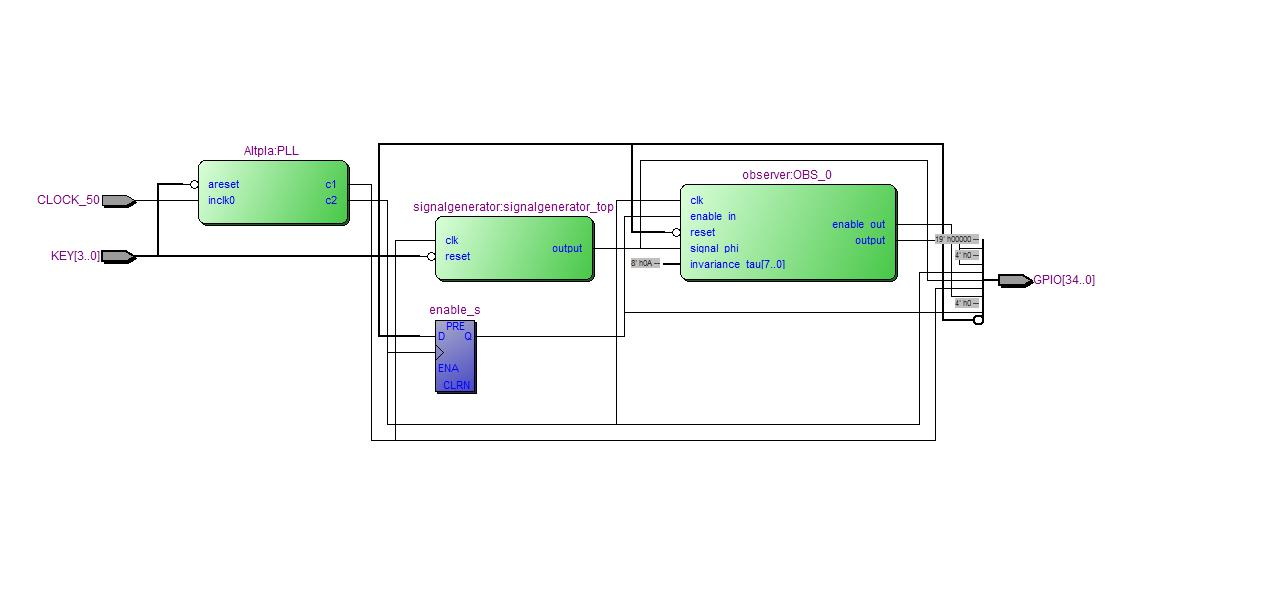
\includegraphics[height]{../../pictures/20.02.2014/TOP.jpg}
\caption[Observer 0 of the Final Version]{Illustration of the Observer 0 from 9 }
\label{fig:version:final:obs:0}
\end{figure}


\begin{figure}[]
\centering
%\hspace{3.0cm}
%\vspace{-5cm}
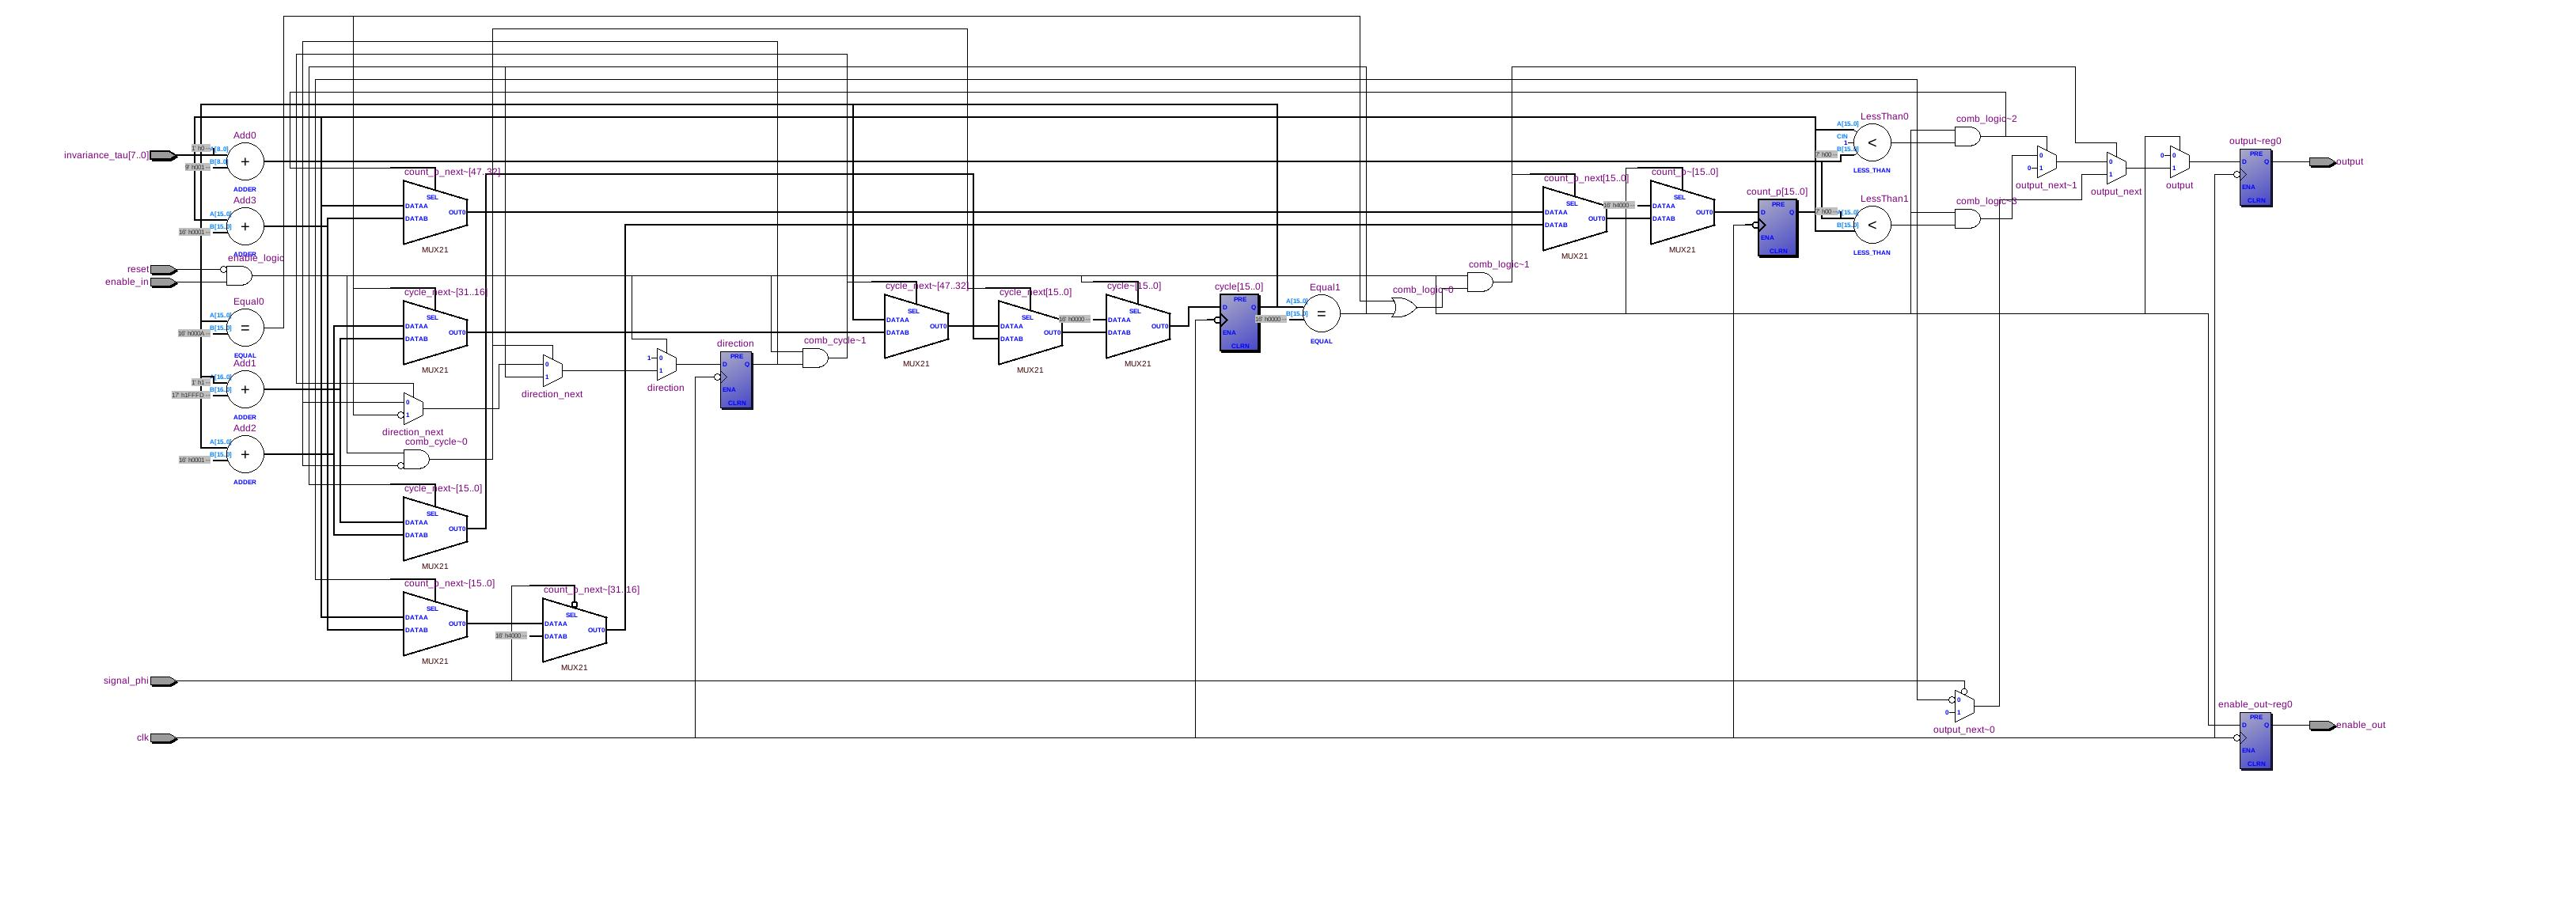
\includegraphics[width=650px,height=300px,angle=-90]{../../pictures/13.06.2014/plain_generator/200Mhz/10OBS/observer_OBS_5.jpg}
%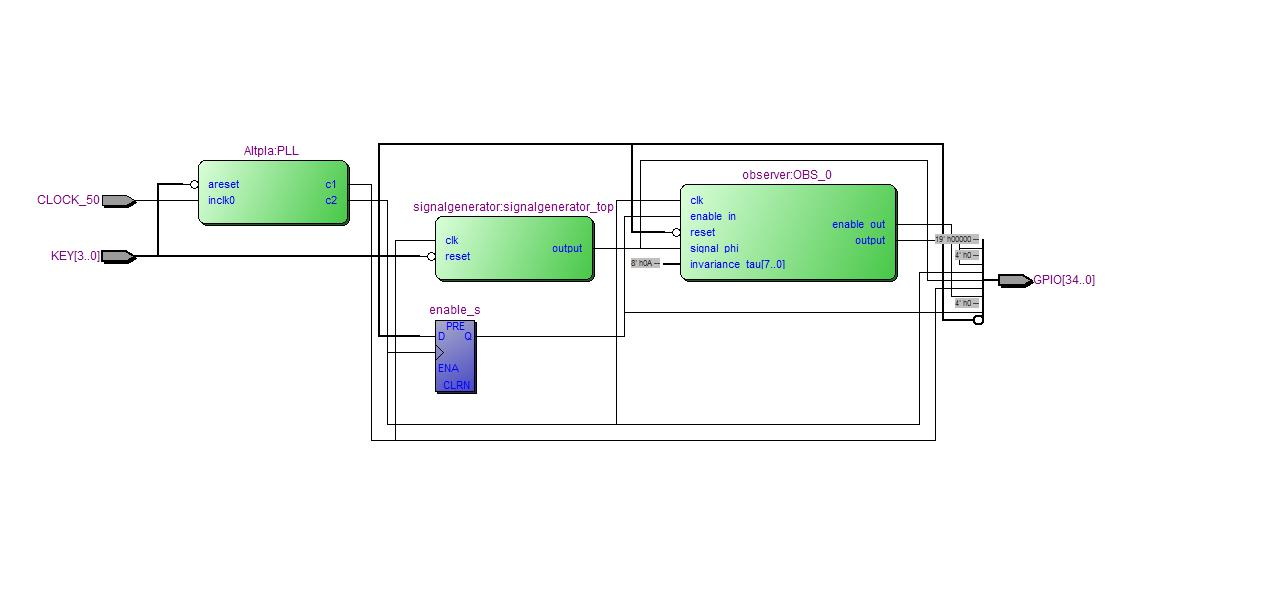
\includegraphics[height]{../../pictures/20.02.2014/TOP.jpg}
\caption[Observer 5  of the Final Version]{Illustration of the Observer 0 from 9 }
\label{fig:version:final:obs:5}
\end{figure}


\begin{figure}[]
\centering
%\hspace{3.0cm}
%\vspace{-5cm}
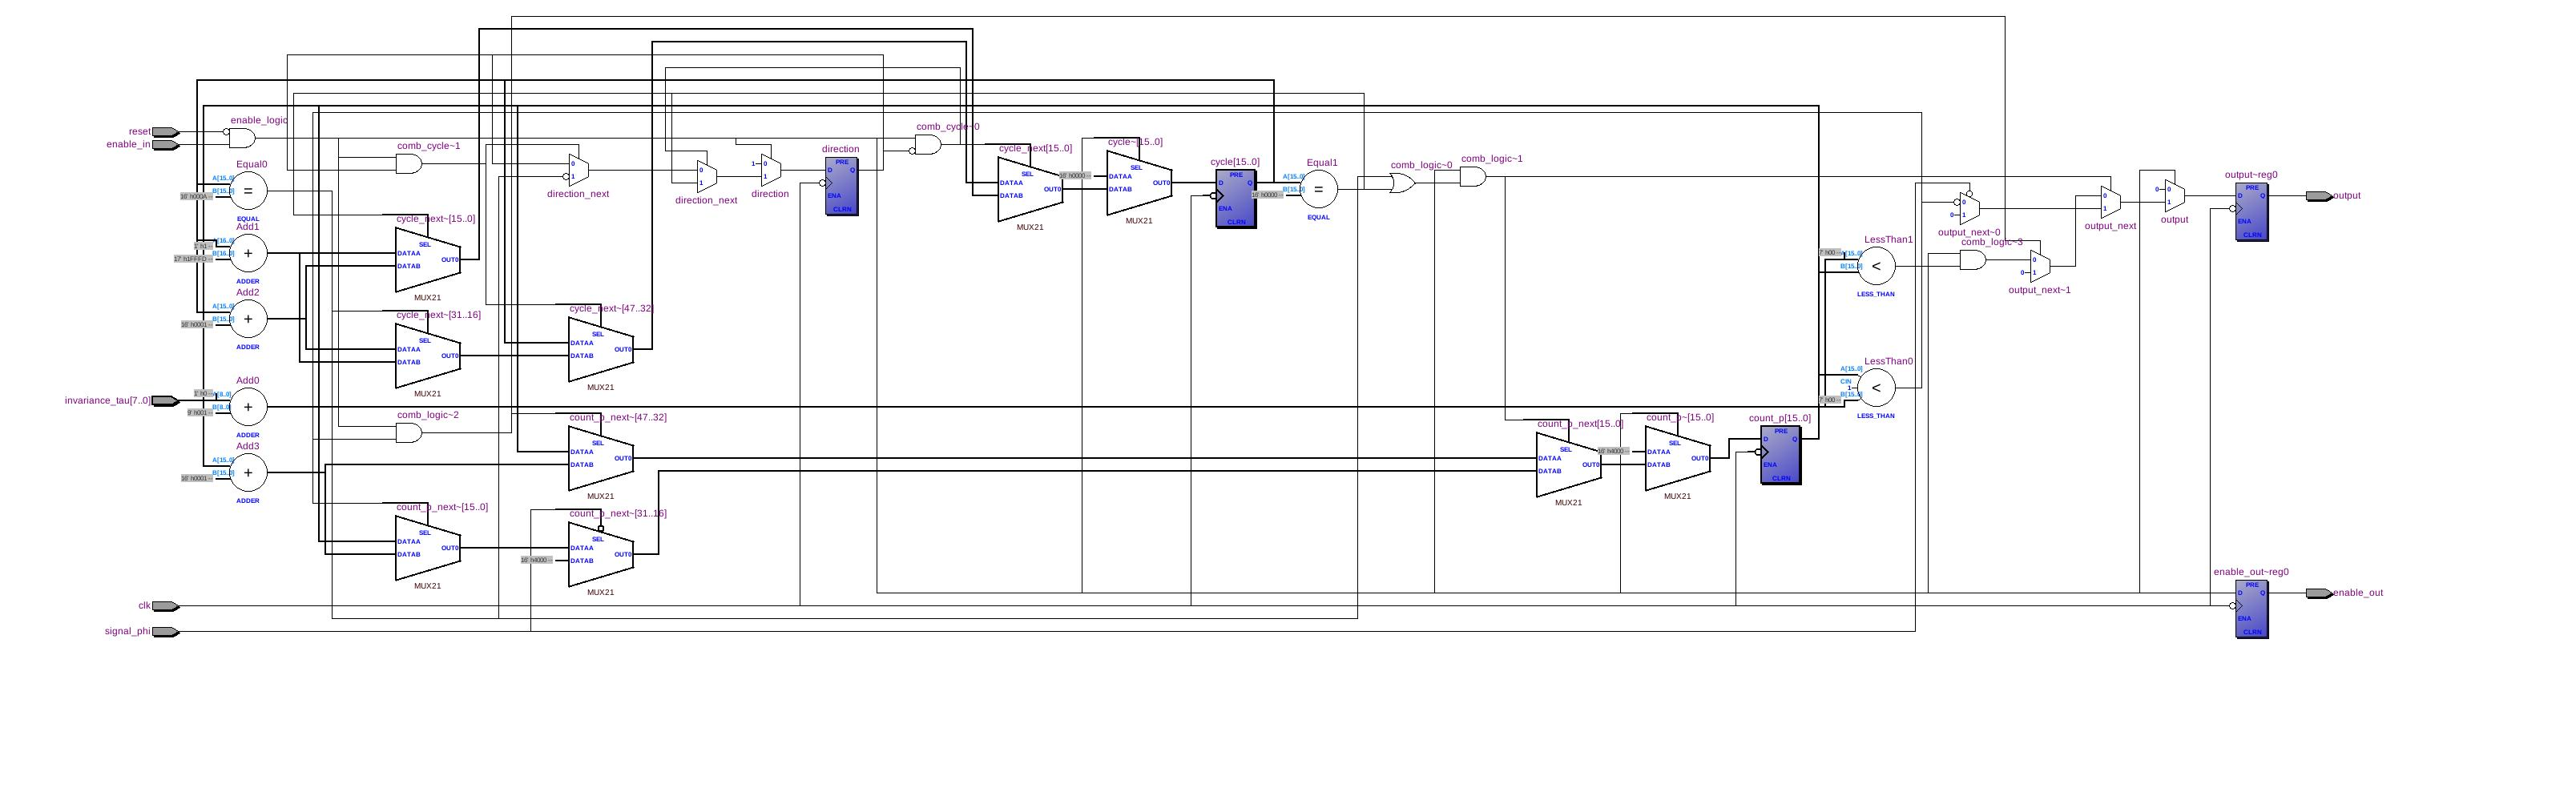
\includegraphics[width=650px,height=300px,angle=-90]{../../pictures/13.06.2014/plain_generator/200Mhz/10OBS/observer_OBS_9.jpg}
%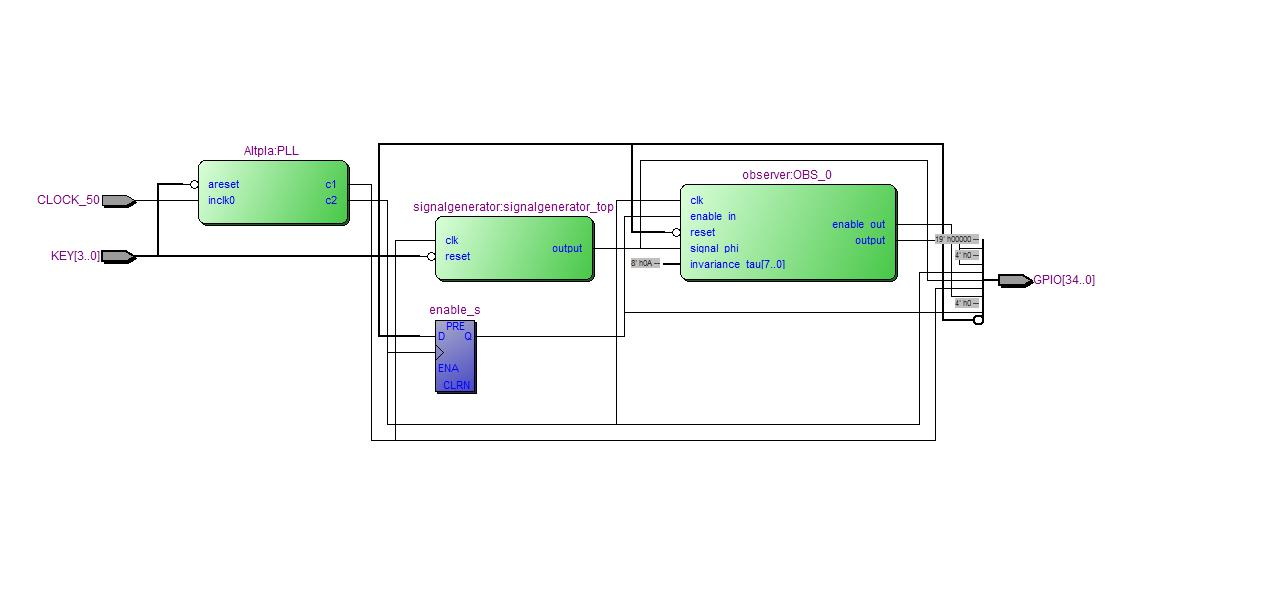
\includegraphics[height]{../../pictures/20.02.2014/TOP.jpg}
\caption[Observer 9  of the Final Version]{Illustration of the Observer 5 from 9 }
\label{fig:version:final:obs:9}
\end{figure}

